\expandafter\ifx\csname ifdraft\endcsname\relax
\documentclass[a4paper,11pt, dvipdfmx]{jreport}
%%%%%%%%%%%%%%%%%%%%余白設定%%%%%%%%%%%%%%%%%%%%
\renewcommand{\baselinestretch}{1.20}
\oddsidemargin  =   5mm \topmargin      =  -5mm
\headsep        =  11mm \headheight     =   7mm
\textheight     = 230mm \textwidth      = 160mm
%%%%%%%%%%%%%%%%%%%%%%%%%%%%%%%%%%%%%%%%%%%%%%%%
 \begin{document}
\fi


%%%%%%%%%%%%%%%%%%%%%%%%%%%%%%%%%%%%%%%%%%%%%%%%%%%%%%%%%%%%%%%%%%%%%%%%%%%%%%%%%%%%%%%%%%%%%%%%%%%%%%%%%%%%%%%%%%%

\def\Path{./4_COP}

%%%%%%%%%%%%%%%%%%%%%%%%%%%%%%%%%%%%%%%%%%%%%%%%%%%%%%%%%%%%%%%%%%%%%%%%%%%%%%%%%%%%%%%%%%%%%%%%%%%%%%%%%%%%%%%%%%%

\chapter{脳波の概要\label{chap:脳波の概要}}

本章では本システムでメンタルを推定する際に利用する脳波の概要について説明を行う.脳波の周波数毎の特徴や脳波の記録方法,脳波とメンタル状態の関係,正常脳波の定義と年齢による特徴,脳波計測におけるアーチファクトについて解説する.
次に脳と機械を接続する技術であるBCIあるいはBMIについて説明を行う.
%----------------------------------------------------------------------------------------------------------------  脳波の周波数帯分類  --------------------------------------------------------------------------------------------------------------%
\section{基礎律動の概要}
脳波は波形として出力され,脳波の大部分を占める特定の脳波活動を基礎律動(basic rhythm)と呼ぶ.基礎律動は,覚醒状態や睡眠状態などの脳の活動レベル,年齢に応じて変化し,個人差も存在する.
基礎律動は周波数の帯域で分類され,$\delta$波,$\theta$波,$\alpha$波,$\beta$波,$\gamma$波の5つに大別される.基礎律動における周波数帯域は脳波に関する分野がまだ未確定であるため,厳密には定まっていない.
一般的には健常者は安静・閉眼状態において,後頭部を中心に8〜13Hzの$\alpha$波が優勢に観測される.睡眠の深さは脳波の周波数帯域の変化と密接に関連しており,睡眠段階の評価において重要な指標となる.
これらの周波数は得られた脳波信号に対して離散フーリエ変換を適用することでそれぞれのパワースペクトルが抽出される.離散フーリエ変換を行うことで得られた$\alpha$波や$\beta$波のパワースペクトル,$\alpha$波や$\beta$波の脳波全体に対する割合,$\alpha$波と$\beta$波の比率などがメンタル状態推定における特徴量として用いられる場合が多い.
$\alpha$波は安静時や覚醒時にみられる波形だが,リラックス状態時には$\alpha$波の振幅が増加する傾向がある.逆に緊張時には$\alpha$波の振幅が減少し,$\beta$波の振幅が増加する傾向がある.
また$\beta$波は,覚醒時の思考活動や問題解決,注意集中時に増加する.$\beta$/$\alpha$波は,ストレスの度合いを評価する指標として用いられることが多い.
基礎率動の各周波数帯の特徴について以下に説明する.

%---------------------------------------------------------------------------------------------------------------- $\delta$波  --------------------------------------------------------------------------------------------------------------%
\subsection{$\delta$波}

$\delta$波は,およそ0.5〜4Hzの低周波数帯に属する脳波であり,主に深い睡眠状態において顕著に観測される.特に,ノンレム睡眠の深い段階では,$\delta$波が優勢となることが知られている.
覚醒時において$\delta$波が増加する場合,極度の疲労,意識レベルの低下,または集中力の著しい低下が生じている可能性が示唆される.そのため,$\delta$波は人間の意識レベルや覚醒度を評価する指標として用いられることがある.
メンタル状態との関係においては,$\delta$波は直接的に感情を反映するというよりも,心身の疲労度や回復状態を示す指標として位置付けられることが多い.

%---------------------------------------------------------------------------------------------------------------- $\theta$波  --------------------------------------------------------------------------------------------------------------%
\subsection{$\theta$波}

$\theta$波は,およそ4〜8Hzの周波数帯に属する脳波であり,浅い睡眠状態や,覚醒と睡眠の中間状態において多く観測される.また,リラックス状態や瞑想状態,あるいは内省的な思考を行っている際にも$\theta$波が増加することが報告されている.
一方で,覚醒時において$\theta$波が過剰に出現する場合,注意力の低下や集中力不足,精神的疲労の兆候である可能性がある.このため,$\theta$波は集中状態と非集中状態を識別する指標とされている.
メンタル状態との関係においては,$\theta$波はリラックスと集中低下の両側面を持つ波形であり,他の周波数帯との相対的な関係を考慮することが重要である.

%---------------------------------------------------------------------------------------------------------------- $\alpha$波  --------------------------------------------------------------------------------------------------------------%
\subsection{$\alpha$波}

$\alpha$波は,およそ8〜13Hzの周波数帯に属する脳波であり,安静覚醒状態において最も典型的に観測される.目を閉じてリラックスしている状態では$\alpha$波が優勢となり,逆に目を開けたり,外部刺激に注意を向けたりすると$\alpha$波は減衰する.
$\alpha$波は,リラックス状態や精神的安定と深く関係しており,ストレスが低く,落ち着いた状態で増加する傾向がある.一方で,過度に$\alpha$波が優勢な状態は,外界への注意が低下している可能性を示す場合もある.
本研究においては,$\alpha$波をメンタルの安定度やリラックス度を評価する重要な指標として扱う.

%---------------------------------------------------------------------------------------------------------------- $\beta$波  --------------------------------------------------------------------------------------------------------------%
\subsection{$\beta$波}

$\beta$波は,およそ13〜30Hzの周波数帯に属する脳波であり,覚醒時の思考活動や問題解決,注意集中時に増加する.学習作業や会話,意思決定を行っている際には,$\beta$波が優勢となることが多い.
一方で,$\beta$波が過剰に出現する状態は,精神的緊張や不安,ストレスの増加を示唆することがある.特に,高周波成分の$\beta$波は,過覚醒状態や焦燥感と関連付けられることが多い.
このように,$\beta$波は集中と緊張の両側面を持つ脳波であり,$\alpha$波や$\theta$波との比率関係がメンタル状態の推定において重要となる.

%---------------------------------------------------------------------------------------------------------------- $\gamma$波  --------------------------------------------------------------------------------------------------------------%
\subsection{$\gamma$波}

γ波は,30Hz以上の高周波の脳波である.γ波は,高度な認知機能や情報処理,学習記憶に関与しているとされており,特に注意集中や感覚統合,意識的認知活動と関連付けられることが多い.
意識や知覚,記憶などの高次認知機能と関連付けられており,物体の特徴と物体特有の情報結合において重要な役割を果たしている.
$\gamma$波に焦点を当てた研究が数多く報告されており,周波数の振幅情報だけではなく位相情報にも注目が集まっている.
局所的な興奮性--抑制性の相互作用は感覚,運動,認知などを形作り局所的な$\gamma$帯に反映される.
以上の各脳波の特徴をまとめると,表\ref{tb:eachfrequency}のようになる.

%---------------  表挿入  ---------------%
\begin{table}[H]
    \begin{center}
    \normalsize
    \caption{各周波数成分範囲}
     \begin{tabular}{|c|c|c|}													\hline	
     タイプ&測定可能データ(Hz)&心理状態								\\	\hline
     $\delta$波&0.5~2.75&夢を見ない不快睡眠,ノンレム睡眠,無意識		\\	\hline
     $\theta$波&3.5~6.75&直感的,創造的,想起,空想,幻想,夢			\\	\hline
     low$\alpha$波&7.5~9.25&リラックス,ただし気だるくはない,平穏意識的		\\	\hline
     high$\alpha$波&10~11.75&リラックスしているが集中している,統合的		\\	\hline
     low$\beta$波&13~16.75&思考,自己および環境の認識					\\	\hline
     high$\beta$波&18~29.75&警戒,動揺								\\	\hline
     low$\gamma$波&31~39.75&記憶,高次精神活動						\\	\hline
     mid$\gamma$波&41~49.75&視覚情報処理							\\	\hline
     \end{tabular}
     \label{tb:eachfrequency}
    \end{center}
   \end{table}
   %---------------  表終了  --------------%

   \section{脳波の記録方法}
   脳波データの取得には,電極を用いた非侵襲的な計測方法が一般的である.非侵襲的な計測方法としては,頭皮上に配置した電極を通じて脳の電気活動を記録する方法が一般的に用いられている.
   頭皮上に接着する電極の位置や数などは,システムの目的や精度要求に応じて選択される.その中でも,代表的な手法として国際臨床脳波学会(IFCN)が提唱する10-20電極法(ten-twenty electrode system)と呼ばれる電極配置法がある.
   脳波は2つの電極間の電位差を測定することで記録されるため,基準電極(リファレンス)と呼ばれる参照点が必要となる.基準電極の選択は,計測の安定性やノイズ耐性に影響を与えるため,慎重に行う必要がある.
   身体の一部に電位的に0の点が存在しており,そこを基準電極(reference electrode)として用いることが多い.例えば,耳たぶや鼻筋,頭頂部などが基準電極として利用されることがある.
   頭皮上に配置される電極は探査電極(exploring electrode)と呼ばれている.探査電極と基準電極との間の電位差とって測定する手法は基準電極導出法(reference derivation)あるいは単極導出法(monopolar derivation)と呼ばれている.
   また,2つの探査電極間の電位差を測定する手法は双極導出法(bipolar derivation)と呼ばれている.
   これらの決められた身体の部位に電極を配置することで,脳波信号の安定した取得が可能となる.もし,基準電極が適切に配置されていない場合,計測される脳波信号に脳波以外の筋電位や心電図などの現象が混入し,判読が難しくなる恐れがある.

   \subsection{10-20電極法}
   国際臨床脳波学会によって推奨されている詳しい計測における電極の配置法である.図2.1に示すように,頭皮上の特定のランドマークを基準にして電極を配置する方法である.
   電極の配置は,前後方向および左右方向に20\%ずつ間隔を空けて配置されることから「10-20電極法」と呼ばれている.

\begin{figure}[H]
    \centering
        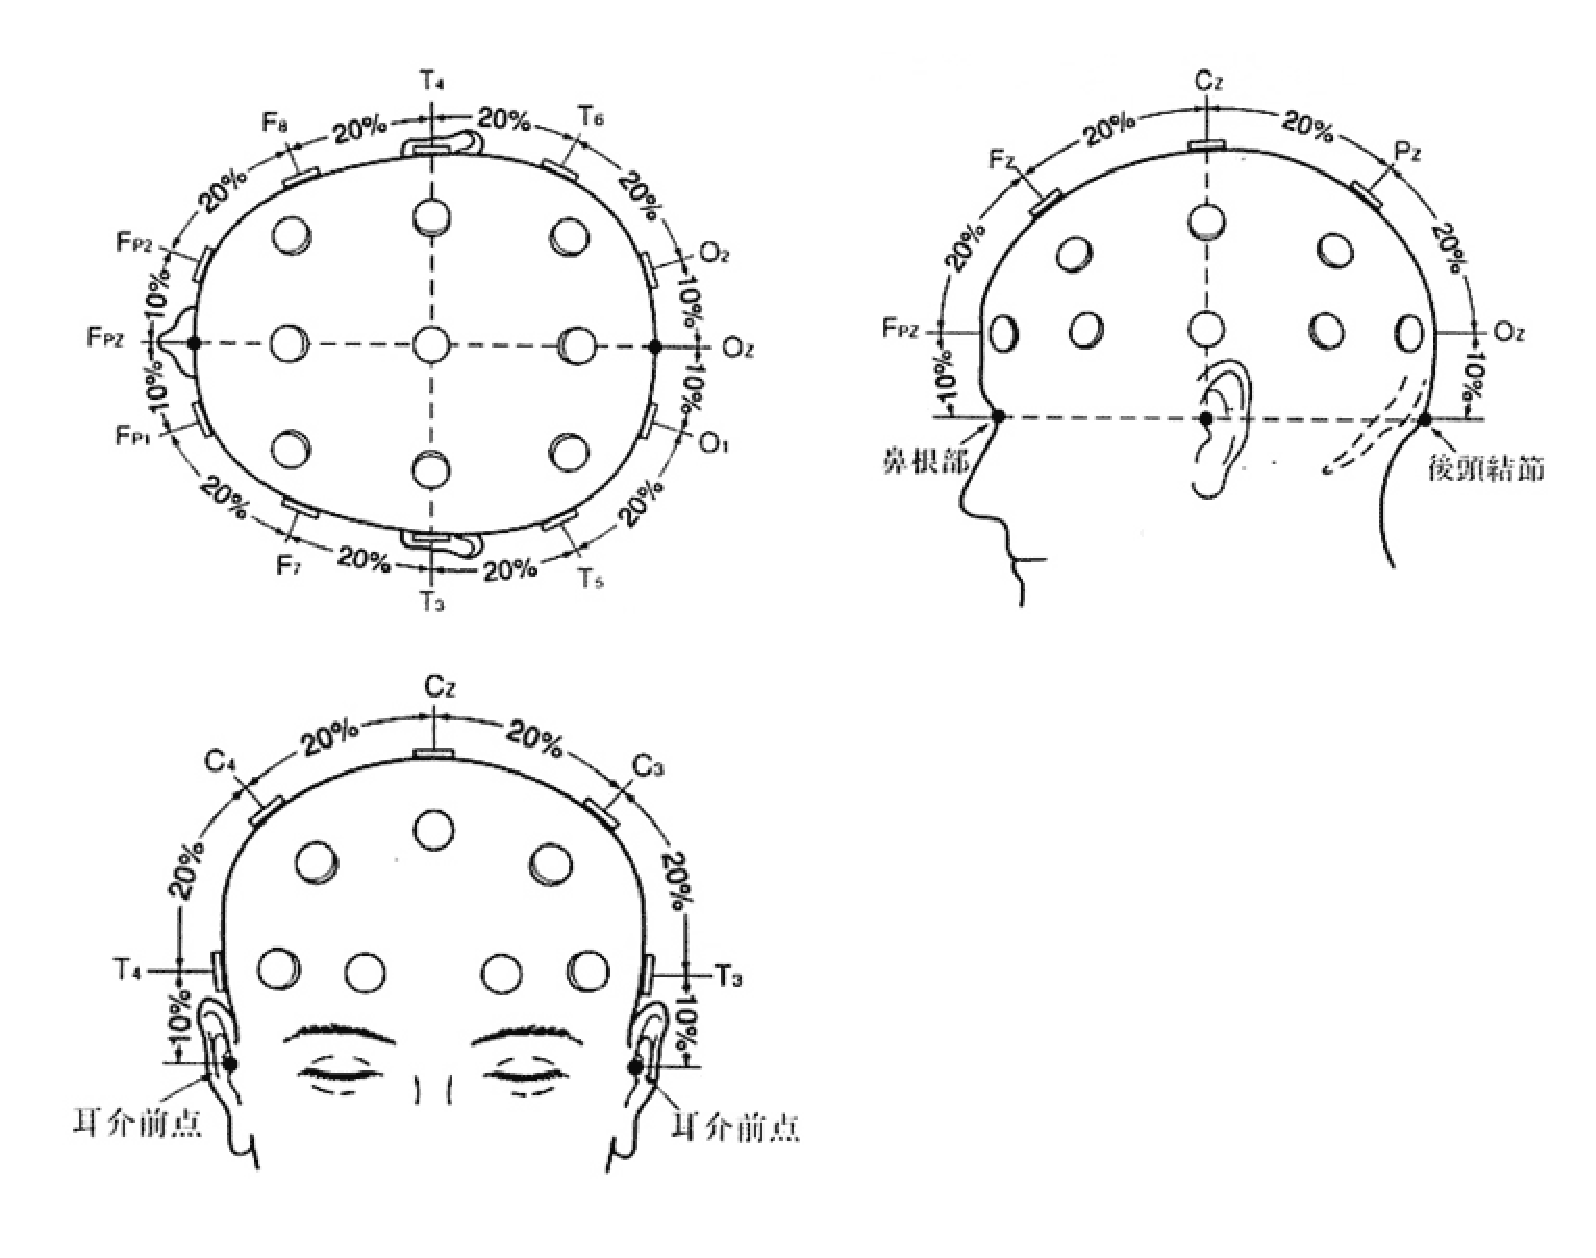
\includegraphics[width=10cm]{./4_COP/Image/10-20system.eps}
        \caption{10-20電極法による電極配置例}
        \label{fig:10-20system}
\end{figure}

\subsection{Gibbs法}
Gibbs法は,脳波信号の空間的な分布を考慮して電極配置を最適化する手法である.この方法では,頭皮上の電極配置を基に,脳波信号の空間的な補間を行い,高解像度な脳波マッピングを実現する.
古くから用いられている方法で,頭皮上に等間隔に配置された12個の探査電極と両耳たぶに配置された2個の基準電極を用いる.

\newpage
\subsection{単極導出法}
単極導出法とは,どちらか一方の電極が電気活動のない電位0の基準点である基準電極に配置され,他方に頭皮上に配置された電位変動のある探査電極である場合の手法である.
基準電極が安定している場所として主に耳たぶと鼻筋が用いられる.

\begin{figure}[H]
    \centering
        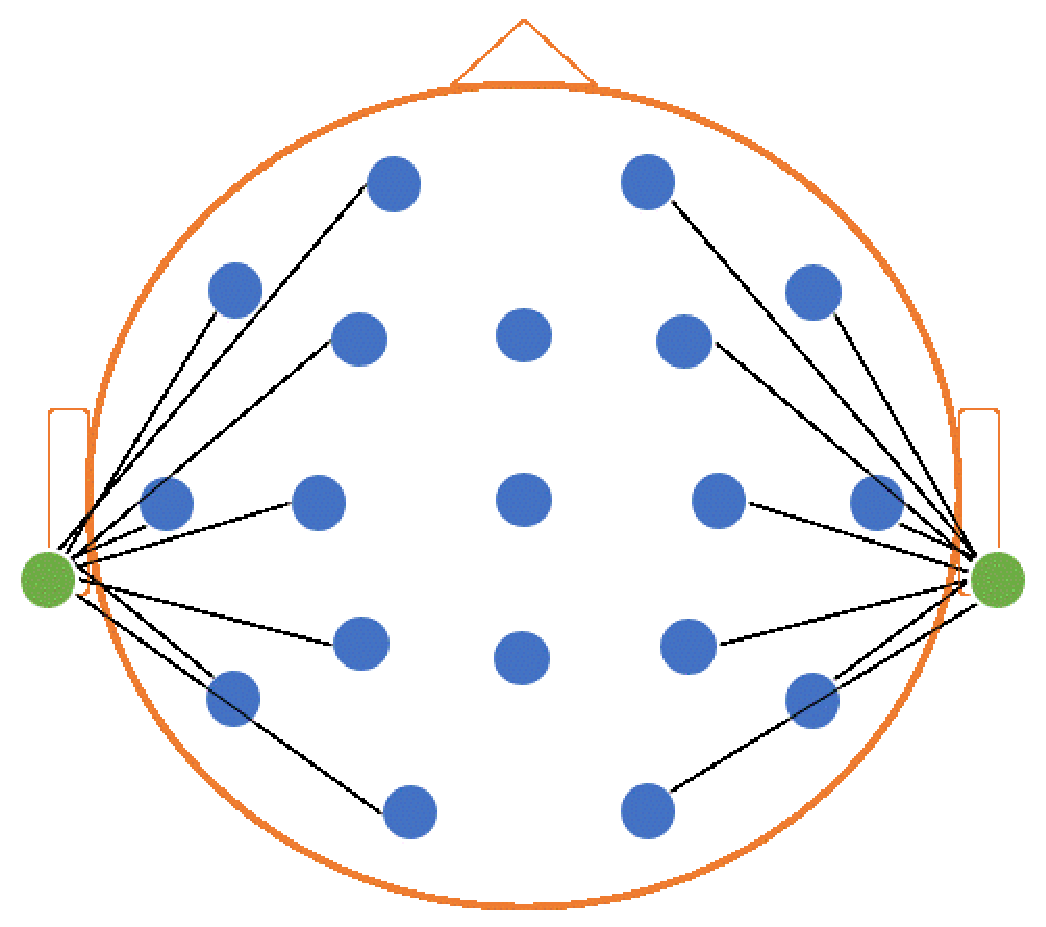
\includegraphics[width=5cm]{./4_COP/Image/tankyoku.eps}
        \caption{単極導出法の概念図}
        \label{tankyoku}
\end{figure}

\subsection{双極導出法}
双極導出法とは,2つの探査電極間の電位差を測定する手法である.この手法では,頭皮上の隣接された2つの探査電極の間の電位差を測定することで,脳波信号を取得する.
双極導出法には,縦の列に配置された電極間で測定を行う縦型双極導出法と,横の列に配置された電極間で測定を行う横型双極導出法がある.以下にそれぞれの概念図を示す.

\begin{figure}[H]
    \centering
        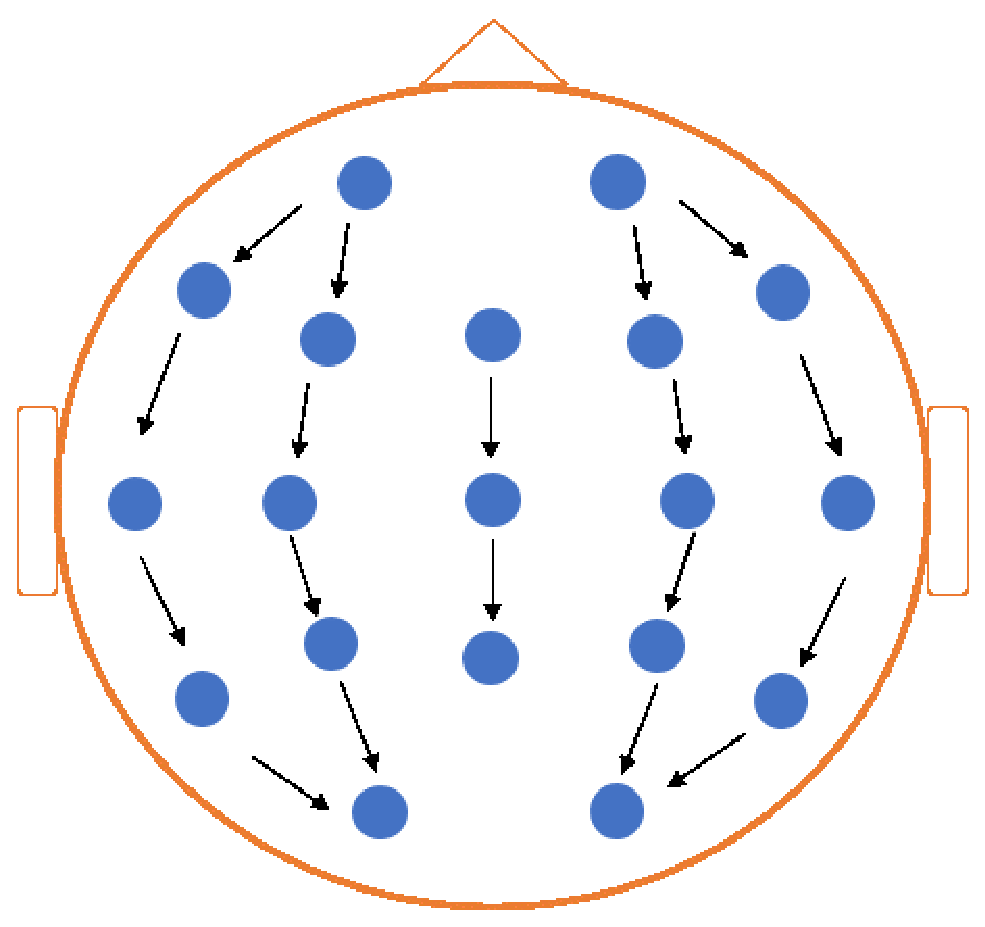
\includegraphics[width=5cm]{./4_COP/Image/soukyoku.eps}
        \caption{縦列双極導出法の概念図}
        \label{soukyoku}
\end{figure}

\begin{figure}[H]
    \centering
        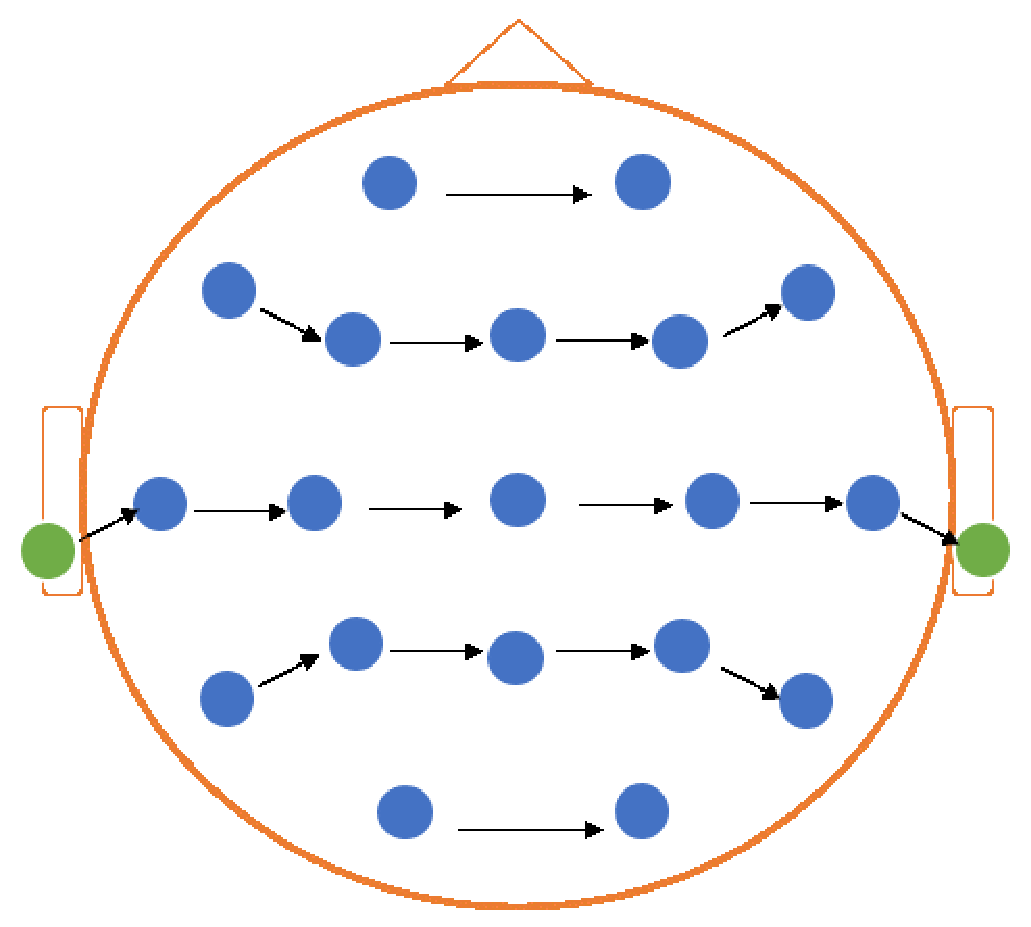
\includegraphics[width=5cm]{./4_COP/Image/soukyoku2.eps}
        \caption{横列双極導出法の概念図}
        \label{soukyoku2}
\end{figure}

\subsection{頭皮電極と脳表電極}
通常は,頭皮上に設置される電極だが,場合によっては,頭蓋骨を開頭し,脳表面に直接電極を配置して脳波を記録することもある.頭皮上の電極では,10-20電極法に電極の配置が従うことが多い.
頭皮上に電極を配置することには,非侵襲的である点と測定機器が比較的安価である点などの利点がある.一方で,頭蓋骨や頭皮を通過する際に信号が減衰し,ノイズの影響を受けやすいという点や,接触不良によるアーチファクトの発生などの欠点も存在する.
脳表電極では,頭蓋骨を開頭し,脳表面に直接電極を配置することで,簡易的な測定は難しいが電ky7億より高精度な脳波信号の取得が可能となる.この方法は,特に難治性てんかんの外科的治療の術前検査などに用いられることが多い.

   %---------------------------------------------------------------------------------------------------------------- 脳波とメンタル状態の関係  --------------------------------------------------------------------------------------------------------------%
\section{脳波とメンタル状態の関係} 
脳波とメンタル状態との関係は,単一の周波数帯のみで評価されるものではなく,複数の周波数成分の相対的なバランスによって特徴付けられる.例えば,$\alpha$波が優勢で$\beta$波が抑制されている状態は,リラックスかつ安定した心理状態を示すと考えられる.一方で,$\beta$波が優勢で$\alpha$波が低下している状態は,強い集中や緊張状態を示す可能性がある.
また,$\theta$波と$\beta$波の比率は,注意力や集中度を評価する指標として用いられることがあり,教育分野や認知研究においても活用されている.これらの比率指標は,個人差が存在するため,絶対値ではなく,相対的変化として扱うことが重要である.
本研究では,脳波の各周波数帯のパワー値およびそれらの比率を特徴量として抽出して機械学習モデルに入力することで,メンタル状態の推定を行う.

%---------------------------------------------------------------------------------------------------------------- 正常脳波の定義と年齢による特徴  --------------------------------------------------------------------------------------------------------------%
\section{正常脳波の定義と年齢による特徴}
正常脳波とは,器質的脳疾患や明らかな神経学的異常が認められない状態において観測される脳波活動を指す.正常脳波は,被験者の年齢,覚醒レベル,精神状態などによって変化するため,一律の波形をもって定義されるものではなく,年齢層ごとの特徴を考慮する必要がある.

%---------------------------------------------------------------------------------------------------------------- 小児における正常脳波の特徴  --------------------------------------------------------------------------------------------------------------%
\subsection{小児における正常脳波の特徴}
小児期における脳波は,成人と比較して低周波成分が優勢であることが特徴である.特に,乳幼児ではδ波や$\theta$波が多く観測され,脳の成熟に伴って徐々に高周波成分が増加していく.
学童期に入ると,$\theta$波の割合が減少し,$\alpha$波が後頭部を中心に出現し始める.しかし,この段階においても成人と比較すると$\alpha$波の周波数はやや低く,振幅が大きい傾向がある.このような特徴は,脳機能が発達途上にあることを反映したものであり,必ずしも異常を示すものではない.

%---------------------------------------------------------------------------------------------------------------- 成人における正常脳波の特徴  --------------------------------------------------------------------------------------------------------------%
\subsection{成人における正常脳波の特徴}
成人における正常脳波では,安静覚醒状態において後頭部優位の$\alpha$波が明瞭に観測されることが一般的である$\alpha$波の周波数は約8〜13Hzの範囲に収まり,左右差が小さいことが正常所見とされる.
覚醒状態での作業や思考時にはβ波が増加し,集中状態と対応する.成人脳波では,これらの周波数帯が状況に応じて柔軟に変化することが特徴であり,脳機能の成熟と安定性を反映している.

%---------------------------------------------------------------------------------------------------------------- 高齢者における正常脳波の特徴  --------------------------------------------------------------------------------------------------------------%
\subsection{高齢者における正常脳波の特徴}
高齢者においては,加齢に伴い$\alpha$波の周波数が低下し,$\theta$波の出現頻度が増加する傾向がある.また,全体的な脳波振幅の低下や,左右差の増大が観測される場合もある.
これらの変化は,加齢に伴う生理的変化として一定範囲内で認められるものであり,必ずしも病的所見を意味するものではない.しかし,$\theta$波や$\gamma$波が過剰に出現する場合には,認知機能低下や脳機能障害の可能性を考慮する必要がある.

%---------------------------------------------------------------------------------------------------------------- 脳波計測におけるアーチファクトの詳細  --------------------------------------------------------------------------------------------------------------%
\section{脳波計測におけるアーチファクトの詳細}
脳波計測では,脳神経活動以外に由来する電気信号が混入することがあり,これらは総称してアーチファクトと呼ばれる.アーチファクトは脳波信号の解釈を困難にし,メンタル状態推定や機械学習モデルの性能低下を招くため,その発生要因と特性を正しく理解することが重要である.

%---------------------------------------------------------------------------------------------------------------- 脈波  --------------------------------------------------------------------------------------------------------------%
\subsection{脈波}
脈波によるアーチファクトは,血管の拍動に伴う微小な電位変動や,頭皮表面の物理的変形によって生じる.特に,電極付近を走行する血管の拍動は,低周波成分として脳波に混入することがある.
このアーチファクトは,心拍数と同期した周期的な波形として現れることが多く,$\gamma$波や$\theta$波帯域と重なるため,覚醒度や疲労状態の評価に影響を及ぼす可能性がある.対策としては,電極の装着位置を工夫することや,心拍データと同期させた信号処理による除去が有効とされている.

%---------------------------------------------------------------------------------------------------------------- 眼球運動  --------------------------------------------------------------------------------------------------------------%
\subsection{眼球運動}
眼球運動によるアーチファクトは,眼球が正負の電位を持つ電気双極子として振る舞うことに起因する.眼球が上下左右に動くことで,前頭部を中心に大きな電位変動が発生し,脳波に混入する.
このアーチファクトは,主に低周波成分として現れ,特に前頭部電極に強く影響する.集中状態やリラックス状態の評価において,$\theta$波や$\alpha$波の誤検出を引き起こす要因となる.計測時には視線移動を最小限に抑えるよう指示し,解析段階ではEOG成分の除去手法を用いることが一般的である.

%---------------------------------------------------------------------------------------------------------------- 発汗  --------------------------------------------------------------------------------------------------------------%
\subsection{発汗}
発汗によるアーチファクトは,皮膚表面の水分量変化に伴い,電極と皮膚間のインピーダンスが変動することで生じる.特に,緊張やストレス状態において発汗が増加すると,脳波信号のベースラインが不安定になる.
この影響は,緩やかな電位ドリフトとして観測されることが多く,低周波帯域の解析に影響を与える.対策としては,電極装着前の皮膚清拭や,長時間計測時における信号の正規化処理が挙げられる.

%---------------------------------------------------------------------------------------------------------------- まばたき  --------------------------------------------------------------------------------------------------------------%
\subsection{まばたき}
まばたきによるアーチファクトは,眼瞼運動に伴う筋電位と,眼球電位変動の複合的な影響によって生じる.まばたき時には瞬間的に大振幅の電位変動が発生し,脳波信号中に鋭いピークとして現れる.
このアーチファクトは,前頭部電極に顕著であり,短時間であっても解析結果に大きな影響を与える可能性がある.解析においては,ピーク検出や独立成分分析などを用いて除去されることが多い.

%---------------------------------------------------------------------------------------------------------------- 不随意運動  --------------------------------------------------------------------------------------------------------------%
\subsection{不随意運動}
不随意運動によるアーチファクトは,筋肉の無意識的な収縮によって生じる筋電位が原因である.特に,顔面筋や首周辺の筋肉は脳波電極に近接しているため,その影響が顕著である.
筋電位は高周波成分を多く含み,β波帯域やそれ以上の周波数帯と重なるため,集中状態や緊張状態の誤判定を引き起こす要因となる.被験者に対してリラックスを促すことや,高周波成分を抑制するフィルタ処理が対策として用いられる.

%---------------------------------------------------------------------------------------------------------------- 体動  --------------------------------------------------------------------------------------------------------------%
\subsection{体動}
体動によるアーチファクトは,被験者の姿勢変化や頭部の動きにより,電極位置がずれたり,電極と皮膚の接触状態が変化することで発生する.
この種のアーチファクトは,突発的かつ大振幅のノイズとして観測されることが多く,解析においてはデータ区間の除外が必要となる場合もある.計測時には,安定した姿勢を保つよう被験者に指示し,装置の固定を十分に行うことが重要である.

%---------------------------------------------------------------------------------------------------------------- 静電誘導  --------------------------------------------------------------------------------------------------------------%
\subsection{静電誘導}
静電誘導によるアーチファクトは,周囲の帯電物体や人体表面の静電気が,電極やケーブルに誘導されることで発生する.特に,乾燥した環境では静電気の影響が顕著になる.
このアーチファクトは,突発的なノイズや基線の揺らぎとして観測されることが多い.対策としては,計測環境の湿度管理や,導電性素材を用いたシールドが有効である.

%---------------------------------------------------------------------------------------------------------------- 電磁誘導  --------------------------------------------------------------------------------------------------------------%
\subsection{電磁誘導}
電磁誘導によるアーチファクトは,周囲の電子機器や電源ケーブルから発生する電磁場が,脳波計測システムに干渉することで生じる.
代表的な例として,商用電源に起因する周期的なノイズが挙げられる.これらは特定周波数に集中して現れるため,ノッチフィルタなどの周波数選択的処理が有効である.

%---------------------------------------------------------------------------------------------------------------- 分極電圧  --------------------------------------------------------------------------------------------------------------%
\subsection{分極電圧}
分極電圧は,電極と皮膚の界面において電気化学反応が生じることで発生する電位差である.この電圧は時間とともに変動し,脳波信号の基線ドリフトを引き起こす.
分極電圧の影響を低減するためには,非分極電極の使用や,適切な電極ジェルの塗布が重要である.

%---------------------------------------------------------------------------------------------------------------- 静電気  --------------------------------------------------------------------------------------------------------------%
\subsection{静電気}
静電気によるアーチファクトは,被験者や周囲環境に蓄積された電荷が放電することで発生する.この影響は,突発的な大振幅ノイズとして現れることが多い.
静電気対策としては,接地の徹底や,合成繊維の使用を避けることが有効である.

%---------------------------------------------------------------------------------------------------------------- 光電効果  --------------------------------------------------------------------------------------------------------------%
\subsection{光電効果}
光電効果によるアーチファクトは,強い光が電極やセンサに照射されることで,光電変換に起因する電流が発生する現象である.特に,光センサと併用する装置では注意が必要である.
このアーチファクトは,照明条件の変化と同期して観測されることがあり,計測環境の光制御が重要となる.

%-------------------------------------------------------------------------------------------------------------------  BCIとBMI  -------------------------------------------------------------------------------------------------------------%

\newpage
\section{BCIとBMI}

急速な科学技術の発達に伴い,多チャンネルかつ高サンプリングにおける環境での脳波計測を実現させ,莫大な情報量のデータを短時間で解析することが可能になった.それにより脳研究は脳機能を解明するためだけではなく,脳活動と工学の技術を合わせた新しい
インターフェースにも応用されつつある.このような脳と機械を相互に接続する技術がブレインコンピュータインターフェース(Brain Computer Interface, BCI)あるいはブレインマシンインターフェース(Brain Machine Interface, BMI)である.
BCIは脳と機械(コンピュータ)を直接つなぎ.脳の命令を身体ではなく機械に入力するシステムである.BCIは考えるだけで機械の操作が行えるようになるため,近未来の技術として注目されている.
BMIとBCIの用語の間に明確な役割はないが.BMIは直接脳の表面あるいは内部に侵襲性の電極を設置する技術を示し,BCIは直接脳を傷つけない非侵襲手法により脳活動を推定する技術を示す場合が多い.
BMIは電極を脳に貼り付けることで,の電気信号を直接計測できるため筋電位などのアーチファクトによる信号汚染が存在しない.
一方BCIは脳内の電気信号を直接計測することはできない,脳信号の精度の観点から比較するとBMIが優れてはいるが,健常者を対象とした利用法を考慮するとBMIは技術的にも倫理的にも多くの問題が存在する.
現状,BMI実験は動物実験か患者に協力を仰ぎ,手術の際に電極を埋め込むという方法でしか実現できない.
また手術には医療的な認可も必要であり,実験を行うために大きな労力と時間とリスクを必要とする.
BMIは気軽に研究することが難しく,一部の大学や研究施設でしか行えない.そのためBMIより精度は落ちるが,一般の人々が脳情報を利用することを考慮するとBCIの発展は必要不可欠である.
BCIは主に非侵襲的な手法で脳と機械を接続する手法である.
数ある非侵襲手法の脳活動計測のなかでも,脳波を利用したBCIが多く研究されている.
一般的に脳波測定は増幅アンプと電極だけで計測が可能であり,大規模な設備も必要なく手軽に計測できる.
実験タスクにおける制限も少なく,日常生活における活動の中で使用可能である.
以下に,脳波を用いた代表的なBCI,BMI研究手法を説明する.


%---------------------------------------------------------------------------------------------------------------- P300スペラー  --------------------------------------------------------------------------------------------------------------
\subsection{P300スペラー}
P300スペラーは,事象関連電位の一種であるP300成分を利用したBCIシステムである.被験者が特定の刺激に注意を向けた際に出現するP300成分を検出し,文字入力などを行うことが可能である.
この方式は,重度運動障害者の意思伝達手段として実用化が進んでおり,比較的少ない学習コストで利用可能である点が特徴である.

%---------------------------------------------------------------------------------------------------------------- 運動出力型BMI  --------------------------------------------------------------------------------------------------------------%
\subsection{運動出力型BMI}
運動出力型BMIは,運動想起に伴う脳波変化を利用して,ロボットアームやカーソルなどを制御する方式である.被験者が手や足の動きを想像することで,対応する脳波パターンが出現し,これを機械学習により識別する.
運動出力型BMIを活用した実験として,脳波計とchatGPTを用いたGmailの操作実験や脳波と言語情報を組み合わせたAIによるロボットアームの遠隔操作実験が報告されている.
この方式は,リハビリテーションや義手制御などへの応用が期待されている.2つの実験の概要を以下の図に示す.

 \begin{figure}[H]
    \centering
        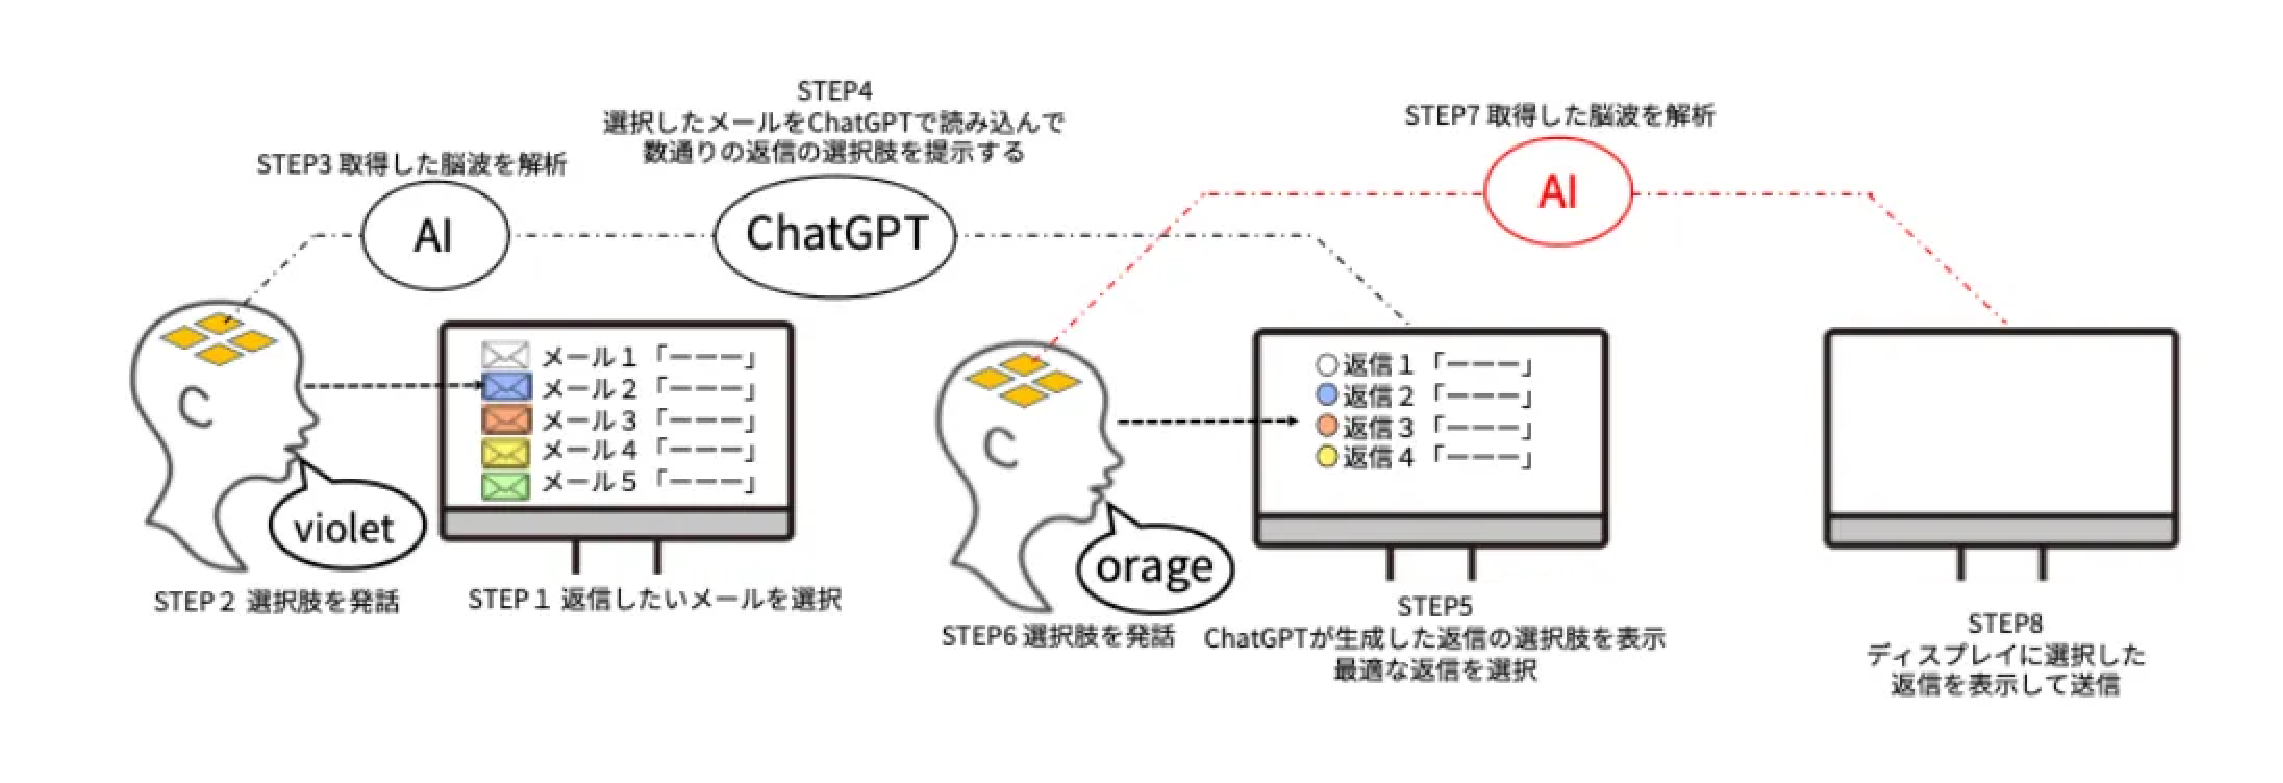
\includegraphics[width=15cm]{./4_COP/Image/BMI1.eps}
        \caption{脳波計とchatGPTを用いたGmailの操作実験の概要}
        \label{fig:10-20system}
\end{figure}

  \begin{figure}[H]
      \centering
          \includegraphics[width=15cm]{./4_COP/Image/BMI2.eps}
          \caption{超高密度脳波計とAIによるロボットアームの遠隔操作実験の概要}
          \label{fig:10-20system}
\end{figure}

%---------------------------------------------------------------------------------------------------------------- 感覚入力型BMIおよび直接操作型BMI  --------------------------------------------------------------------------------------------------------------%
\subsection{感覚入力型BMIおよび直接操作型BMI}
感覚入力型BMIは,外部刺激を脳へフィードバックすることで感覚を補完または拡張する技術である.一方,直接操作型BMIは,脳活動を用いて外部機器を直感的に操作することを目的とする.
これらの技術は,人間と機械の関係性を大きく変える可能性を持ち,本研究におけるAIエージェントとの相互作用設計にも示唆を与えるものである.
運動出力型BMIと同様に,リハビリテーションや義手制御などへの応用が期待されている.以下に,感覚入力型BMIおよび直接操作型BMIの概要図を示す.

\begin{figure}[H]
      \centering
          \includegraphics[width=15cm]{./4_COP/Image/mirai202209_img02.jpg}
          \caption{感覚入力型BMIおよび直接操作型BMIの概要}
          \label{fig:10-20system}
\end{figure}


\expandafter\ifx\csname ifdraft\endcsname\relax
\bibliography{\path bib-TSPS}
\bibliographystyle{jplain}  %% junsrt
  \end{document}
\fi